\documentclass[a4paper,twoside,10pt]{article}
\interfootnotelinepenalty=10000
\usepackage[USenglish]{babel} %francais, polish, spanish, ...
\usepackage[T1]{fontenc}
%\usepackage[ansinew]{inputenc}
\usepackage{color}
\usepackage{mathtools}
%\usepackage{hyperref}
\usepackage{subfig}
\usepackage{multirow, booktabs}
\usepackage{hyperref}


\usepackage{lmodern} %Type1-font for non-english texts and characters
\usepackage{algorithm}
\usepackage[noend]{algpseudocode}
\usepackage{mnsymbol}

%% Packages for Graphics & Figures %%%%%%%%%%%%%%%%%%%%%%%%%%
\usepackage{graphicx} %%For loading graphic files
\usepackage{amsmath}
\usepackage{amsthm} 
\usepackage{thmtools}
\usepackage{amsfonts}
\usepackage[all,cmtip]{xy}
\usepackage{tikz}

\usepackage{TechFront}
%\declaretheorem{Lemma}
%\declaretheorem{prop}

\newcommand{\lre}{\color{red}{\{}}

%\DeclareMathOperator{\sign}{sgn}
%\DeclareMathOperator{\coef}{coef}
%\DeclareMathOperator{\var}{var}
%\DeclareMathOperator{\eqs}{eqs}
%\DeclareMathOperator{\feas}{feas}
%\DeclareMathOperator{\UB}{UB}
%\DeclareMathOperator{\lb}{lb}
%\DeclareMathOperator{\FMcomb}{FM-comb}
%\DeclareMathOperator{\Gcomb}{Gauss-comb}
%\DeclareMathOperator{\proj}{proj}
%\DeclareMathOperator{\Pos}{Pos}
%\DeclareMathOperator{\Neg}{Neg}
%\DeclareMathOperator{\rhs}{rhs}
\newcommand{\sign}{\mathit{sgn}}
\newcommand{\coef}{\mathit{co}}
\newcommand{\var}{\mathit{var}}
\newcommand{\VAR}{\mathit{VAR}}
\newcommand{\eqs}{\mathit{eqs}}
\newcommand{\feas}{\mathit{feas}}
\newcommand{\UB}{\mathit{UB}}
\newcommand{\UBc}{\mathit{UBineq}}
\newcommand{\lb}{\mathit{lb}}
\newcommand{\lbc}{\mathit{lbineq}}
\newcommand{\FMcomb}{\mathit{FM}}
\newcommand{\Gcomb}{\mathit{GA}}
\newcommand{\proj}{\mathit{proj}}
\newcommand{\Pos}{\mathit{Pos}}
\newcommand{\Neg}{\mathit{Neg}}
\newcommand{\rhs}{\mathit{rhs}}
\newcommand{\bounds}{\mathit{bounds}}
\newcommand{\ie}{\mathcal{IE}}
\newcommand{\xx}{\mathcal{X}}
\newcommand{\vea}{\mathbf{co}}
\newcommand{\ttt}{\texttt{t}}
\newcommand{\trt}[1]{\texttt{#1}}
\newcommand{\mi}{\mathit}

\newcommand{\false}{\texttt{false}}
\newcommand{\true}{\texttt{true}}
\newcommand{\nul}{\texttt{null}}
\newcommand{\ve}{\mathbf}
%\newcommand\lhs[1]{\text{lhs}(#1)}
%\newcommand\rhs[1]{\text{rhs}(#1)}
%\newcommand\coef[1]{\text{coef}(#1)}
%\newcommand\LB[1]{\text{LB}_{#1}}
%\newcommand\UB[1]{\text{UB}_{#1}}
\newcommand{\lig}[4]{\ve{#1}\cdot\ve{#2}#3#4}
\newcommand\red[1]{\textcolor{red}{#1}}
\newcommand\blue[1]{\textcolor{blue}{#1}}
\newcommand{\set}[2]{\{\;{#1}\;|\;{#2}\;\}}
\newcommand{\odef}{\overset{\text{def.}}=}
\newcommand{\mc}{\mathcal}
\algdef{SE}[DOWHILE]{Do}{doWhile}{\algorithmicdo}[1]{\algorithmicwhile\ #1}%
\newcommand{\argmin}{\operatornamewithlimits{argmin}}
\newcommand{\StateInd}{\State\hspace{\algorithmicindent}}
\newcommand{\pr}{\mathit{PR}}
\newcommand{\prs}{\mathit{PRS}}
\newcommand{\ens}{\Leftrightarrow}

%\algdef{SE}[DOPAR]{DoPar}{doParWhile}{\algorithmicdo\textbf{ in parallel for\ }}[1]{\algorithmicwhile\ #1}%
\algdef{SE}[DOPAR]{DoPar}{doParUntil}{\algorithmicdo\textbf{ in parallel for\ }}[1]{\algorithmicuntil\ #1}%

\algdef{SE}[SUBALG]{Indent}{EndIndent}{}{\algorithmicend\ }%
\algtext*{Indent}
\algtext*{EndIndent}

\newtheorem{prop}{Proposition}
\newtheorem{lemma}{Lemma}
\newtheorem{cor}{Corollary}

\newcounter{para}
%\newcommand\mypara[1]{\par\refstepcounter{para}\textbf{\thep‌​ara\space#1\space}}
\newcommand\mypara[1]{\newline\par\refstepcounter{para}\textbf{\thepara}\space \textbf{#1} \space}
%\newcommand\mypara{\par\refstepcounter{para}\thepara\space}
%\usepackage[thmmarks,...]{ntheorem}
\newcommand{\Sec}{F}
\newcommand{\Ca}{\mi{Cap}}
\newcommand{\Vol}{\mi{V}}
\newcommand{\Weight}{\mi{W}}
\newcommand{\weight}{\mi{w}}
\newcommand{\BonjeanStations}{\mi{BS}}
\newcommand{\bonjean}{bf}
\newcommand{\Bonj}{B}
\newcommand{\shear}{\mi{sf}}
\newcommand{\Prop}{P}

\theoremstyle{definition}
%\newtheorem{example}{Example}[section]
\newtheorem*{theorem}{Theorem}

\theoremstyle{definition}
\newtheorem{examplex}{Example}[section]
\newenvironment{example}
  {\pushQED{\qed}\renewcommand{\qedsymbol}{$\triangle$}\examplex}
  {\popQED\endexamplex}
	
%\newtheoremstyle{named}{}{}{\itshape}{}{\bfseries}{.}{.5em}{\thmnote{#3}}
%\theoremstyle{named}
%\newtheorem*{namedtheorem}{Theorem}

\begin{document}
\section*{Appendix}
\subsection*{Vessel data}
The vessel's data is given by the following sets and constants.

\vspace{1mm}
\noindent
\begin{tabular}{p{1.8cm}p{4cm}|p{1.3cm}p{4.5cm}}
\multicolumn{2}{l}{\textbf{Sets used in vessel data}}\\
\hline\noalign{\smallskip}
$L$  & Locations. &
$T$	 & Types of containers.\\ 
$S$	 & Sections. (Ordered set)&
$T^\trt{20}\subseteq T$ & Types that are $20'$ long. \\
$S^\trt{f}, S^\trt{a}\subseteq S$ & Sections fore/aft. &
$T^\trt{R}\subseteq T$ & Types that are reefers.\\
$L_s\subseteq L$ & Locations in section $s\in S$ &
$\mi{BT}$ & Ballast tanks. \\
$F$	 & Frames. &
$B$ & Blocks with constant weight.\\
$ST$ & Stations. 
\end{tabular}

\vspace{1mm}
\noindent
$ST$ includes $\sigma^\trt{a}$ and $\sigma^\trt{f}$, which are two (artificial) stations at the aft most and fore most positions of the ship, respectively. Similarly, $F$ contains the frames $f^\trt{a}$ and $f^\trt{f}$. The areas (bounds) for these stations (frames), are trivial.

It is assumed that if $L_s\neq \emptyset$ then $L_s$ contains all locations that are positioned within some interval on the longitudinal axis.    
%$\forall s\in S\forall l\in L: \min\set{P^\trt{a}_{l'}}{l'\in L_s}\leq l \leq\max\set{P^\trt{f}_{l'}}{l'\in L_s} \Rightarrow l\in L_s$.}

\vspace{1mm}
\noindent
\begin{tabular}{p{4.5cm}p{8cm}}
\multicolumn{2}{l}{\textbf{Constants used in vessel data}}\\
\hline\noalign{\smallskip}
$C_l^\trt{20}$, $C_l^\trt{40}$, $C_l^\trt{TEU}$, $C_l^\trt{RS}$, $C_l^\trt{RC}$, 
$C_l^\trt{W20}$, $C_l^\trt{W40}\in \mathbb{N}$ & The capacity for each location $l\in L$, w.r.t. $20'$ containers, $40'$ container, TEUs, reefer slots, reefer cells, weight of $20'$ containers, and weight of $40'$ containers, respectively.\\
$W_\tau, W_b\in \mathbb{R}$ & The weight of a type of container $\tau\in T$, and of a block $b\in B$, respectively. \\
$A_{\sigma,d}\in \mathbb{R}^+_0$ & The area submerged in water at station $\sigma\in ST$ for some displacement $d$ in a finite set $D$.\\
$P^\trt{f}_l, P^\trt{a}_l, P^\trt{f}_b, P^\trt{a}_b, P^\trt{f}_t, P^\trt{a}_t\in\mathbb{R}$ & The longitudinal position of the fore and aft endpoint of location $l\in L$, block $b \in B$ and tank $t \in BT$, respectively.\\
$P_\sigma, P_f\in \mathbb{R}$& The lengthwise position of station $\sigma\in ST$, and of frame $f\in F$, respectively.\\
$\mi{Max}^\trt{wTotal}$, $\mi{Max}^\trt{t}_b\in \mathbb{R}^+$& Upper bound for the total displacement and for each ballast tank $b\in BT$, respectively.\\
$\mi{Max}^\trt{sf}_f$, $\mi{Min}^\trt{sf}_f$, $\mi{Max}^\trt{bm}_f$, $\mi{Min}^\trt{bm}_f\in\mathbb{R}$ & The upper and lower bounds for the shear force and bending moment at each frame $f\in F$, respectively.\\
\end{tabular}


\subsection*{Output data and vessel model}
In the Vessel Model, buoyancy data and hydrostatic constraints are translated to sections end points. 

The Vessel Model uses the sets $L$, $S$, $T$, $T^{\trt{20}}, T^\trt{R}$ and $BT$ (given above), while the used variables are summarized in Table~\ref{table:constants}. Our standard model uses the constants $C_s^\trt{20}$, $C_s^\trt{40}$, $C_s^\trt{TEU}$, $C_s^\trt{RS}$, $C_s^\trt{RC}$, 
$C_s^\trt{W20}$, $C_s^\trt{W40}$, $W_\tau$ and $\mi{Max}^\trt{wTotal}$ (given above) as well as the constant given in Table~\ref{table:constants}. The constants from Table~\ref{table:constants} are calculated from the input data as explained further below.

Regarding the variables, we note that even though $x_{l,\tau}$ is a number of containers and hence a natural number, we model it as a reel number to ensure that the resulting model is an LP.  

%the for and aft thing - for a middle point, do we sum fore or aft for sf and bm. I think its ok, I might just have defined S^a and S^f generically
\begin{table}
\centering
\begin{tabular}{p{3.5cm}p{9cm}}
\multicolumn{2}{l}{\textbf{Decision variables}}\\
\hline
$x_{l,\tau}\in \mathbb{R}^+_0$
		&Number of containers of each type $\tau\in T$ to be stowed in each location $l\in L$.\\
$xt_s\in \mathbb{R}^+_0$
		& The weight of ballast tanks within section $s\in S$.\\
\\
\multicolumn{2}{l}{\textbf{Auxilliary variables}}\\
\hline
$x_\tau\in \mathbb{R}^+_0$ & The total number of containers of each type $\tau\in T$.\\
$w_s\in \mathbb{R}^+_0$	& The weight of section $s\in S$, everything included.\\
$\mi{wTotal}\in \mathbb{R}^+_0$	& The total displacement.\\
$b_{s,d} \in\mathbb{R}$ & The buoyancy force for section $s \in S$ with a total displacement of $d\in \mathbb{R}$.\\
$\mi{sf}_s\in \mathbb{R}$ & The shear force at the aft endpoint of each section $s\in S$.\\
$\mi{bm}_s\in \mathbb{R}$ & The bending moment at the aft endpoint of each section $s\in S$.\\
%
\multicolumn{2}{l}{\textbf{Constants}}\\
\hline\noalign{\smallskip}
$P^\trt{f}_s$, $P^\trt{a}_s \in \mathbb{R}$ & The fore and aft position of each section $s \in S$.\\  
$\mi{Max}^\trt{sf}_s$, $\mi{Min}^\trt{sf}_s$, $\mi{Max}^\trt{bm}_s$, $\mi{Min}^\trt{bm}_s \in \mathbb{R}$ & The upper and lower bounds for the shear force and bending moment at the aft endpoint of each section $s\in S$.\\
$\mi{Max}^\trt{t}_s\in \mathbb{R}$ & The upper bound for the weight of ballast tanks in section $s\in S$.\\
\end{tabular}
\caption{Variables and constants used to describe the Vessel Model. $C_s^\trt{20}$, $C_s^\trt{40}$, $C_s^\trt{TEU}$, $C_s^\trt{RS}$, $C_s^\trt{RC}$, $C_s^\trt{W20}$, $C_s^\trt{W40}$, $W_\tau$ and $\mi{Max}^\trt{wTotal}$ from the input data is used as well.}\label{table:constants}
\end{table}
%
\subsubsection*{Constraints}
\paragraph{Location-based capacity constraints}
Firstly, we have constraints that ensure that for each location of the vessel, the stowed containers are within the allowed capacities w.r.t. the number of $20'$ containers, $40'$ containers, TEUs, and the weight of the $20'$ and $40'$ containers, respectively. These constraint are modeled in the inequalities \eqref{20Cap}-\eqref{weight40Cap} below.
{Likewise, we have a constraint, \eqref{combinedWeightCap}, that ensures that the weight of a location is within limits, taken the different distribution of the weight of $40'$ containers, respectively $20'$ containers, within a slot into consideration; the weight of a $40'$ container is distributed on the four outer corner places of a slot while the weight of $20'$ containers also rest on the inner corners of the slot.}
Lastly, \eqref{reeferSlotCap} and \eqref{reeferCellCap} ensure that each reefer container can be refrigerated, and that {the total number of cells taken up by the reefer containers are within capacity}, respectively. 
\begin{align}
{\forall l \in L:}&\quad
	\label{20Cap}
	{\sum_{\tau \in T^\trt{20}} x_{l,\tau} \leq C_l^\trt{20} }\\
	%
	\label{40Cap}    	
	{\forall l \in L:}&\quad
	{\sum_{\tau \in T\setminus T^\trt{20}} 2\cdot x_{l,\tau} \leq C_l^\trt{40} }\\
	%
	\label{teuCap}
	\forall l \in L:&\quad
	\sum_{\tau \in T^\trt{20}} x_{l,\tau} + 2\cdot\sum_{\tau \in T\setminus T^\trt{20}} x_{l,\tau} \leq C_l^\trt{TEU}\\
	%
	\label{weight20Cap}
	\forall l \in L:&\quad
	\sum_{\tau \in T^\trt{20}} W_\tau\cdot x_{l,\tau} \leq C_l^\trt{W20}\\
	%
	\label{weight40Cap}
	\forall l \in L:&\quad\sum_{\tau \in T\setminus T^\trt{20}} W_\tau\cdot x_{l,\tau} \leq C_l^\trt{W40} \\
	%
	\label{combinedWeightCap}
	\forall l \in L:&\quad 0.5\cdot \sum_{\tau \in T^\trt{20}} W_\tau\cdot x_{l,\tau} + \sum_{\tau T\setminus \in T^\trt{20}		} W_\tau\cdot x_{l,\tau} \leq C_l^\trt{W40}\\
	%
	\label{reeferSlotCap}
	\forall l \in L:&\quad\sum_{\tau \in T^\trt{R}} x_{l,\tau} \leq C_l^\trt{RS} \\
	%
	\label{reeferCellCap}
	{\forall l \in L:}&\quad
	{\sum_{\tau \in T^\trt{20R}} 0.5\cdot x_{l,\tau} + \sum_{\tau \in T^\trt{40R}} x_{l,\tau} \leq C_l^\trt{RC} }
\end{align}	 
%

The constraint in \eqref{typeDef} defines the variables, $x_\tau$, that specifies how many containers of a specific type $\tau$ is stowed on the vessel. These are the variables that we want the projected (in)equality system to be expressed in.
\begin{equation}
\label{typeDef}
	\forall{\tau \in T}: x_\tau = \sum_{l\in L} x_{l,\tau}
\end{equation}

For defining the weight of a section, we need its fore and aft posiiton. For \emph{cargo-containing sections}, i.e. sections $s$ for which $L_s\neq \emptyset$, we can find immediate fore- and aft points of the locations/bays in $s$: $P^\trt{if}_s = \max\set{P^\trt{f}_l}{l\in L_s}$, and $P^\trt{ia}_s = \min\set{P^\trt{a}_l}{l\in L_s}$ (see Figure~\ref{fig:sections}). 
There is a small gap between two consecutive bays, and this space is divided evenly between two consecutive, cargo-containing sections, such that the aft end point of the fore-most section aligns with the fore end point of the aft-most section. Sections that are not cargo-containing get their endpoints from the immediate end points of their neighbour-sections if these are cargo-containing, and otherwise the non-cargo containing parts of the vessel is divided evenly among the corresponding non-cargo-containing sections. See Figure~\ref{fig:sections}.

\begin{figure}
	\centering
		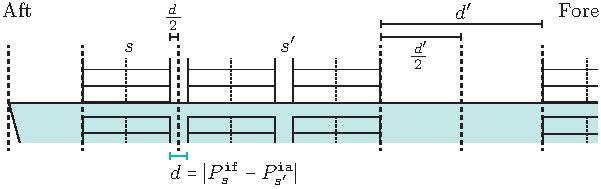
\includegraphics{C:/Users/ajspur/FMEarticle/figures/sections.pdf}
	\caption{The doted lines indicates the endpoints of the sections.}
	\label{fig:sections}
\end{figure}

Using the end points of the sections, \eqref{totalWeightDef} below defines the total weight of section $s\in S$, including cargo, ballast tanks and the vessel itself.   

\begin{equation}
\label{totalWeightDef}
	\forall s \in S:\quad w_s = \sum_{\tau \in T} W_\tau\cdot\sum_{l\in L_s} x_{l,\tau} + xt_s + \sum_{b\in B} \mi{percent}([P^\trt{a}_b;P^\trt{f}_b],[P^\trt{a}_s;P^\trt{f}_s])\cdot W_b,
\end{equation}
where $\mi{percent}(J, I)$ defines how big a percentage of the interval $J=[J_1; J_2]$ lies within the interval $I = [I_1; I_2]$. That is, 
\[
\mi{percent}([J_1;J_2], [I_1; I_2]) = \frac{\max(\min(J_2, I_2)-\max(J_1, I_1),0)}{I_2-I_1}.
\]
We also ensure that the number of containers of each type placed in each location, as well as the amount of ballast in the ballast tanks within each section is positive. 
For the ballast tanks, we also require that each tank's content is within limits, and likewise for the the total weight (displacement). These constraints are given in \eqref{xPos}, \eqref{btLim}, and \eqref{wTotalLim} below.
\begin{align}
	\label{xPos}
	\forall l\in L, \tau\in T:&\quad 0 \leq x_{l,\tau}.\\
	%
	\label{btLim}
	\forall s \in S:	&\quad 0 \leq xt_s \leq \mi{Max}(xt_s) := \sum_{b \in BT} \mi{percent}([P_b^\trt{a};P_b^\trt{f}],[P_s^\trt{a};P_s^\trt{f}])\cdot \mi{Max}^\trt{t}_b\\
%
	\label{wTotalLim}
	&\quad \sum_{s\in S} w_s \leq \mi{Max}^\trt{Wtotal}
\end{align}
\paragraph{Hydrostatic constraints}
At each station $\sigma$ the submerged area of the cross-section for a given displacement $d$ in a discrete set of values, $D$, is given by $A_{\sigma,d}$. 
We make the assumption that above a given treshold $d_{min}\in D$ (and until the maximal displacement $d_{max}$ given in $D$), the submerged area is close to a linear function of the displacement. The submerged area $A'_{\sigma,d}$ for any $d\in [d_{min};d_{max}]$ can therefore be approximated as 
\[
A'_{\sigma,d} = \frac{A_{\sigma,d_{max}} - A_{\sigma,d_{min}}}{d_{max} - d_{min}} \cdot (\mi{wTotal} - d_{max}) + A_{\sigma,d_{max}},
\]
and we extend this to hold for every $d\in \mathbb{R}$.

The submerged area between two consecutive stations $\sigma$ and $\sigma'$ are linearized, so that the submerged area for displacement $d$ at any point $p\in[P_\sigma;P_{\sigma'}]$, where $\sigma\neq \sigma^\trt{f}$ and $\sigma' = \mi{argmin}_{\set{s}{P_s > P_\sigma}}P_s$, is approximated by
\[
A''_{p,d} = \frac{A'_{\sigma',d}-A'_{\sigma,d}}{P_{\sigma'}-P_\sigma}\cdot(p-P_\sigma) + A'_{\sigma,d}.
\]

From this we can calculate the buoyancy of section $s \in S$ at a displacement $d\in \mathbb{R}$. First we let $P := \{P^\trt{a}_s, P^\trt{f}_s\} \cup \set{P_\sigma}{\sigma\in ST,\; P^\trt{a}_s < P_\sigma < P^\trt{f}_s}$ be the points of the stations between (and including) the section's two endpoints. Then the buoyancy of the section $s$ is given by
\[
b_{s,d} = \sum_{p \in P\setminus \{P^\trt{f}_s\}} \frac{1}{2}\cdot(A''_{p,d}+A''_{\mi{next}_p,d})\cdot (\mi{next}_p-P), \text{where } \mi{next}_p = \min\set{p' \in P}{p' > p}.
\]
In a similar manner, we linearize the upper bound for the shear force between two consecutive frames, so that the upper bounds for the shear force at the aft endpoints of section $s$ is
\[
\mi{Max}^\trt{sf}_s = \frac{\mi{Max}^\trt{sf}_{f_2}-\mi{Max}^\trt{sf}_{f_1}}{P_{f_2}-P_{f_1}}\cdot(P^\trt{a}_s - P_{f_1}) + \mi{Max}^\trt{sf}_{f_1}, 
\]
where $f_1 = \mi{argmax}_{\set{f\in F}{P_f\leq P^\trt{a}_s}}P_f$ and $f_2 = \mi{argmax}_{\set{f\in F}{P_f>P^\trt{a}_s}}P_f$. Of course, if there is an $f\in F$ such that $P^\trt{a}_s = P_f$ then we let $\mi{Max}^\trt{sf}_s = \mi{Max}^\trt{sf}_f$. Similarly we find $\mi{Min}^\trt{sf}_s$, as well as for $\mi{Max}^\trt{bm}_s$ and $\mi{Min}^\trt{bm}_s$.   

The shear forces at each section $s$'s aft endpoint can then be calculated. If $s\in S^\trt{f}$ ($s\in S^\trt{a}$), then the shear force at the aft endpoint equals the total weight $w_s$ of the sections fore (aft) $P^\trt{a}_s$ minus the (positive) buoyancy of the sections fore (aft) $P^\trt{a}_s$, this is given in \eqref{sf} below. For each of the sections, we then require these shear forces to be within limits (\ref{sfLim}).   

Similarly, the bending moment at section $s$'s aft endpoint is calculated as the sum of resulting forces of sections $s'$ ($w_{s'} - b_{s', \mi{wTotal}}$) lying fore (aft) $P^\trt{a}_s$ times the distance from $P^\trt{a}_s$ to $s'$'s (longitudinal) midpoint (\ref{bm}). Naturally, these values are then required to lie within the calculated limits (\ref{bmLim}).

\begin{gather}
\label{sf}
\forall s \in S:\;
\mi{sf}_s = \sum_{s' \in S'_s} (w_{s'} - b_{s',wTotal}),\\
\nonumber \text{where }S'_s = \left\{
\begin{array}{ll} \set{s' \in S^\trt{f}}{P^\trt{f}_{s'} \geq P^\trt{f}_s}&\text{if }s \in S^\trt{f}\\
									\set{s' \in S^\trt{a}}{P^\trt{a}_{s'} < P^\trt{a}_s}&\text{if }s \in S^\trt{a}\end{array}\right..
\\
\label{sfLim}\forall s \in S:\;
\mi{Min}^\trt{sf}_s \leq \mi{sf}_s \leq \mi{Max}^\trt{sf}_s\\
%
\label{bm}\forall s \in S:\;
\mi{bm}_s = 	\sum_{s' \in S'_s} (w_{s'} + b_{s',wTotal})\cdot |P^\trt{a}_s - \frac{P^\trt{f}_{s'}-P^\trt{a}_{s'}}{2}|\\
%
\label{bmLim}
\mi{Min}^\trt{bm}_s \leq \mi{bm}_s \leq \mi{Max}^\trt{bm}_s. 
\end{gather}
\end{document}